% !TEX root = Master.tex



As mentioned in Section \autoref{ssec:data_sources}, our data contains the information about sold articles over the years 2017 and 2018. \autoref{fig:total_sold_articles_ts} shows the weekly course for the quantities over those two years, highlighting active promotion weeks as vertical lines. We can undoubtedly recognize that \textit{"Black Friday"} weeks (black lines) have an exceptional impact on sales, as they stand internationally for the most busy shopping periods. During these days in mid- to late November each year, large amounts of different products are heavily discounted.\\

\begin{figure}[H]
\centering
  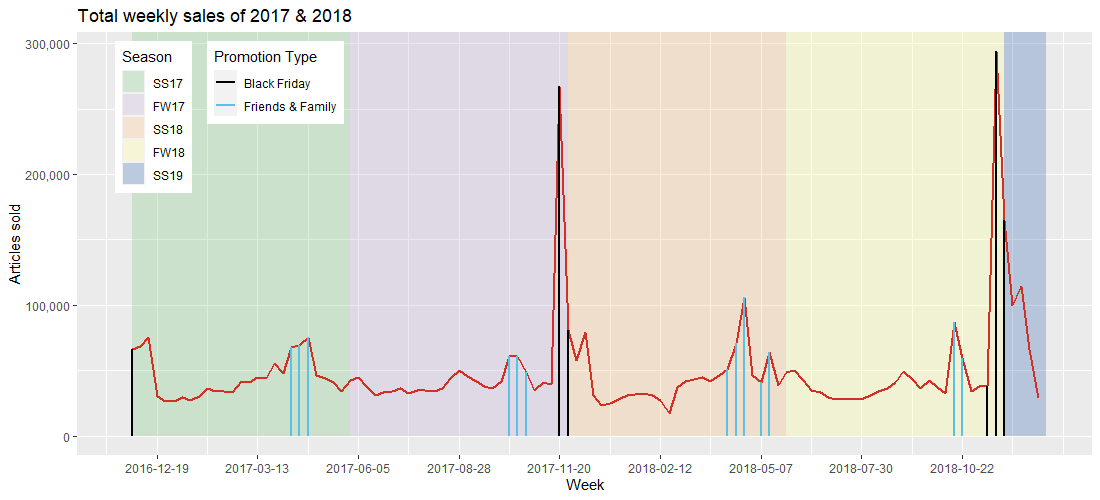
\includegraphics[width=1\linewidth]{figures/total_sold_articles_ts.png}
  \caption{Course of article unit sales}
  \label{fig:total_sold_articles_ts}
\end{figure}

Another promotion type we are interested in is \textit{"Friends \& Family"}, occurring yearly around April-May and October, where on the eCom website plenty of articles are on offer. On these weeks, we have elevated numbers of sold articles as well(\autoref{fig:total_sold_articles_ts}, blue lines). Tables \ref{tab:black_friday} and \ref{tab:friends_and_family} show the weeks were Black Friday and Friends \& Family took place respectively. The dates indicate always the Monday of the respective week (we assume that a week starts on Monday). \\


\begin{table}[H]
\setlength\arrayrulewidth{1pt}  
\centering
\begin{adjustbox}{max width=\textwidth}

\
\begin{tabular}{|
>{\columncolor{lightgray}}c |c|c|c|c|c|c|}
\hline
\textbf{Black Friday weeks} & 2016-11-28 & 2017-11-20 & 2017-11-27 & 2018-11-12 & 2018-11-19 & 2018-11-26 \\ \hline
\end{tabular}

\end{adjustbox}
\caption{Black Friday weeks}
\label{tab:black_friday}
\end{table}




\begin{table}[H]
\setlength\arrayrulewidth{1pt}  
\centering
\begin{adjustbox}{max width=\textwidth}

\
\begin{tabular}{|
>{\columncolor{lightgray}}c |c|c|c|c|c|c|c}
\hline
\cellcolor{lightgray}                                              & 2017-04-10 & 2017-04-17 & 2017-04-24 & 2017-10-09 & 2017-10-16 & 2017-10-23 & \multicolumn{1}{l|}{2018-04-09} \\ \cline{2-8} 
\multirow{-2}{*}{\cellcolor{lightgray}\textbf{Friends \& Family weeks}} & 2018-04-16 & 2018-04-23 & 2018-05-07 & 2018-05-14 & 2018-10-15 & 2018-10-22 &            \\ \cline{1-7}
\end{tabular}

\end{adjustbox}
\caption{Friends \& Family weeks}
\label{tab:friends_and_family}
\end{table}


Excluding the months of the two mentioned promotion types, they don't seem to have a very large impact on sales. The monthly sales portions for those months can be observed in \autoref{fig:sales_without_promo_months}. We have slightly higher sales portions on January, June and July. Most probably this is due to Christmas and "end of the year" shopping habits, which are carried forward from December to the very next month January. Regarding June and July, they indicate summer periods and frequent occurrence of big sports events, which may drive sales as well. 
Notice that, despite the fact that December is not explicitly present in \autoref{tab:black_friday}, it is nonetheless a Black Friday month as the promotion is still activated moving from November to December (see \autoref{fig:monthly_ts}). \\


 \begin{figure}[H]
\centering
\begin{subfigure}{.45\textwidth}
  \centering
  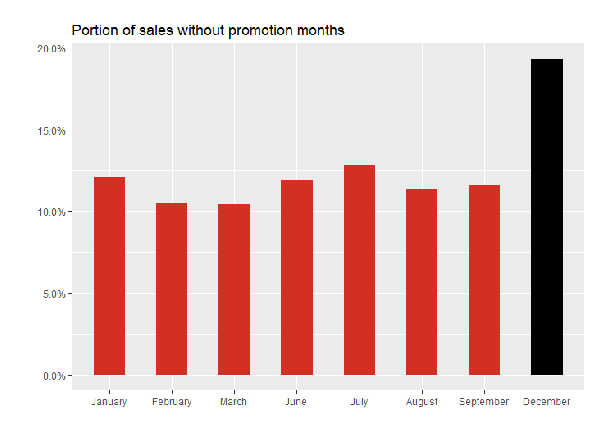
\includegraphics[width=\linewidth]{figures/sales_without_promo_months.eps}
  \caption{Sales distribution grouped by months without promos}
  \label{fig:sales_without_promo_months}
\end{subfigure}
\begin{subfigure}{.45\textwidth}
  \centering
  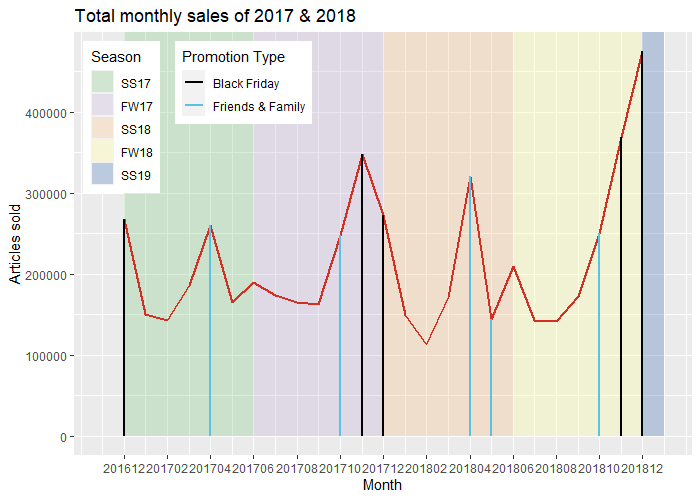
\includegraphics[width=\linewidth]{figures/monthly_ts.png}
  \caption{Monthly course of article unit sales with promo indicators}
  \label{fig:monthly_ts}
\end{subfigure}
\caption{Monthly patterns of article unit sales}
\label{fig:monthly_sales}
\end{figure}



Moving forward, reviewing some sales summary statistics along with the findings so far, we detect a very high overdispersion in our data. The first two rows in \autoref{tab:quantiles_sold_units_week} give as a first impression of the sales distribution. Considering the sold units of one article at a time within a week, there are lots of weeks where no single unit was sold. The median is at 2.71 units,\footnote{Reminder from Section \ref{ssec:data_sources}: the values are in reality discrete, but due to anonymization the were transformed into real numbers.} 75\% of the "article-week" combinations take on a value of at most 20 and the minority exceeds 100 pieces (99\%-quantile). The third row of the table shows how many distinct articles fall under the respective quantile of sales and there is a visible anti-proportional behaviour towards the number of sold units, which is of course intuitive. Remarkable though is the quantity of affected articles even for incredibly large quantiles.\\


\begin{table}[H]
\setlength\arrayrulewidth{1pt}  
\centering
\begin{adjustbox}{max width=\textwidth}\
 \begin{tabular}{|
>{\columncolor{lightgray}}c |c|c|c|c|c|c|c|c|c|}
\hline
\textbf{Quantile}             & Min   & 25\%  & 50\%  & 75\%  & 90\%  & 95\%  & 99\%   & 99.9\% & Max \\ \hline
\textbf{\# Sold units / week} & 0     & 0.45  & 2.71  & 8.14  & 19.45 & 34.39 & 102.71 & 360.12 & 6,816.74 \\ \hline
\textbf{\# Affected articles} & 26,203 & 26,195 & 23,797 & 17,014 & 10,275 & 6,458  & 1,800   & 273  & 1  \\ \hline
\end{tabular}
\end{adjustbox}
\caption{Number of sold units per week \& number of affected articles for various quantiles of sales}
\label{tab:quantiles_sold_units_week}
\end{table}


Conscientiously, we want to inspect the number of weekly sold units above and below a certain (large) threshold to find out how promotions influence these vast sales numbers. In \autoref{fig:bar_below_200_units_week} we can see how the sales are distributed over Black Friday, Friends \& Family and regular weeks for below a threshold of 200 units. Most high sales occurrences don't enjoy any promotion, making the search of cause more difficult for these extreme cases. Observations above that threshold of 200 can be seen in \autoref{fig:bar_above_200_units_week} and we can clearly see a change from the previous figure. As expected, Black Friday is the dominating promotion type, although this the majority remains in not promoted sales, making search of causation for extreme observations not trivial.\\


 
 \begin{figure}[H]
\centering
\begin{subfigure}{.45\textwidth}
  \centering
  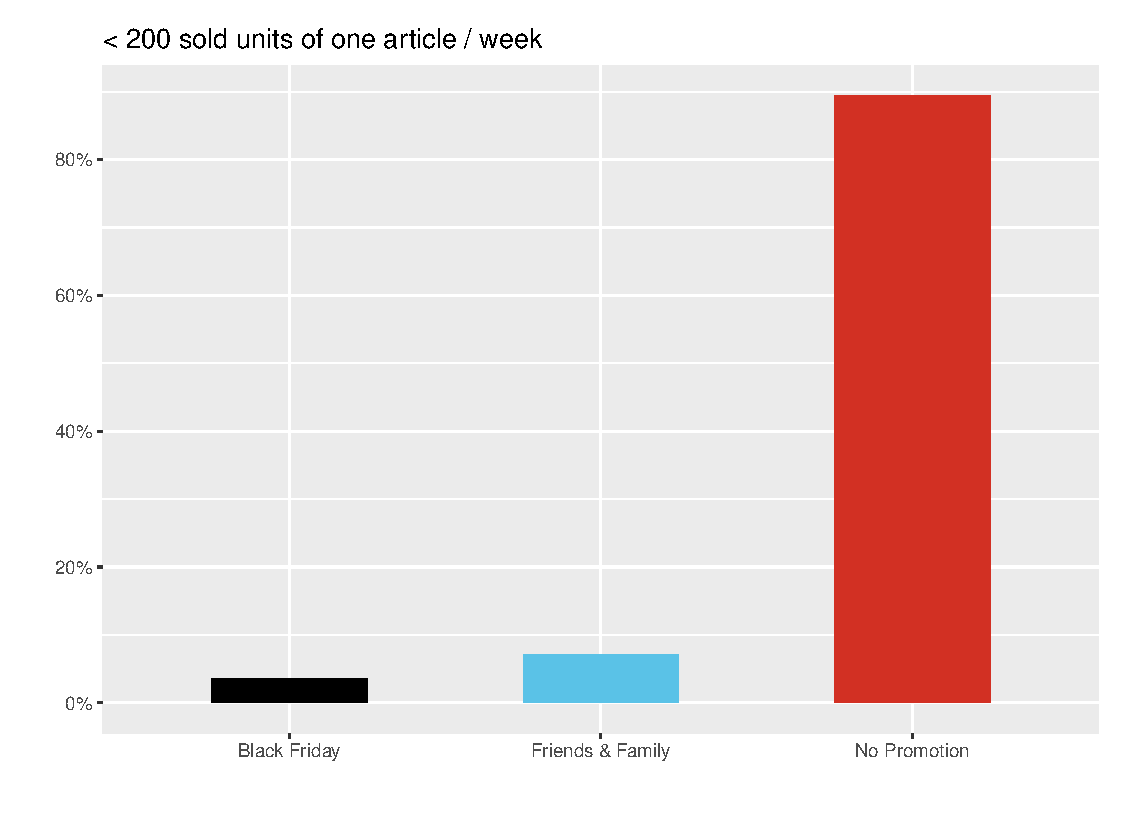
\includegraphics[width=\linewidth]{figures/bar_below_200_units_week.eps}
  \caption{Below 200 units}
  \label{fig:bar_below_200_units_week}
\end{subfigure}
\begin{subfigure}{.45\textwidth}
  \centering
  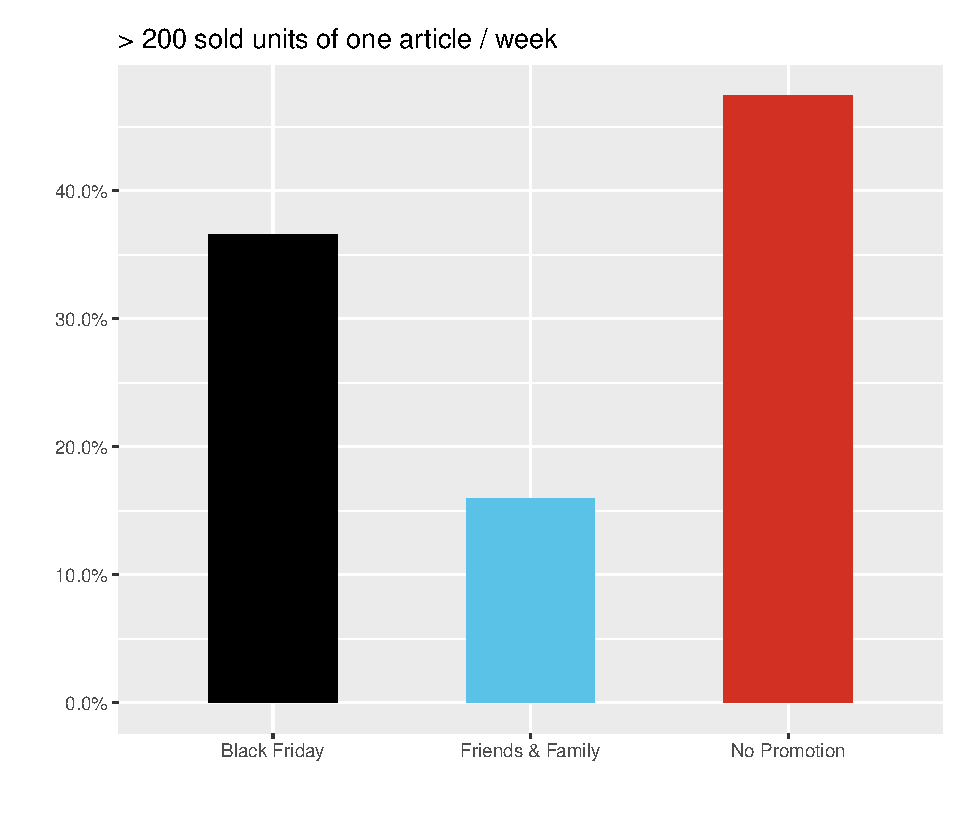
\includegraphics[width=\linewidth]{figures/bar_above_200_units_week.eps}
  \caption{Above 200 units}
  \label{fig:bar_above_200_units_week}
\end{subfigure}
\caption{Distribution of sold units of articles per week split at 200 units}
\label{fig:200_split_plots}
\end{figure}


To validate our exploration on this, we may look at the empirical \ac{CDF} in \autoref{fig:ecdf_all} using all observations now.
Instances with no promotions have a steeper curve (red line) and reach their maximum faster compared to articles tagged with a promotion in a certain week. The less concave curve of Friends \& Family promoted sales (blue line) implies that there are more instances with a larger amount of sold units overall. The same behaviour is even more pronounced for Black Friday (black line), having considerably more high quantity instances. Along these lines, promotions might somewhat explain this pattern better.\\
 
 
 \begin{figure}[H]
\centering
  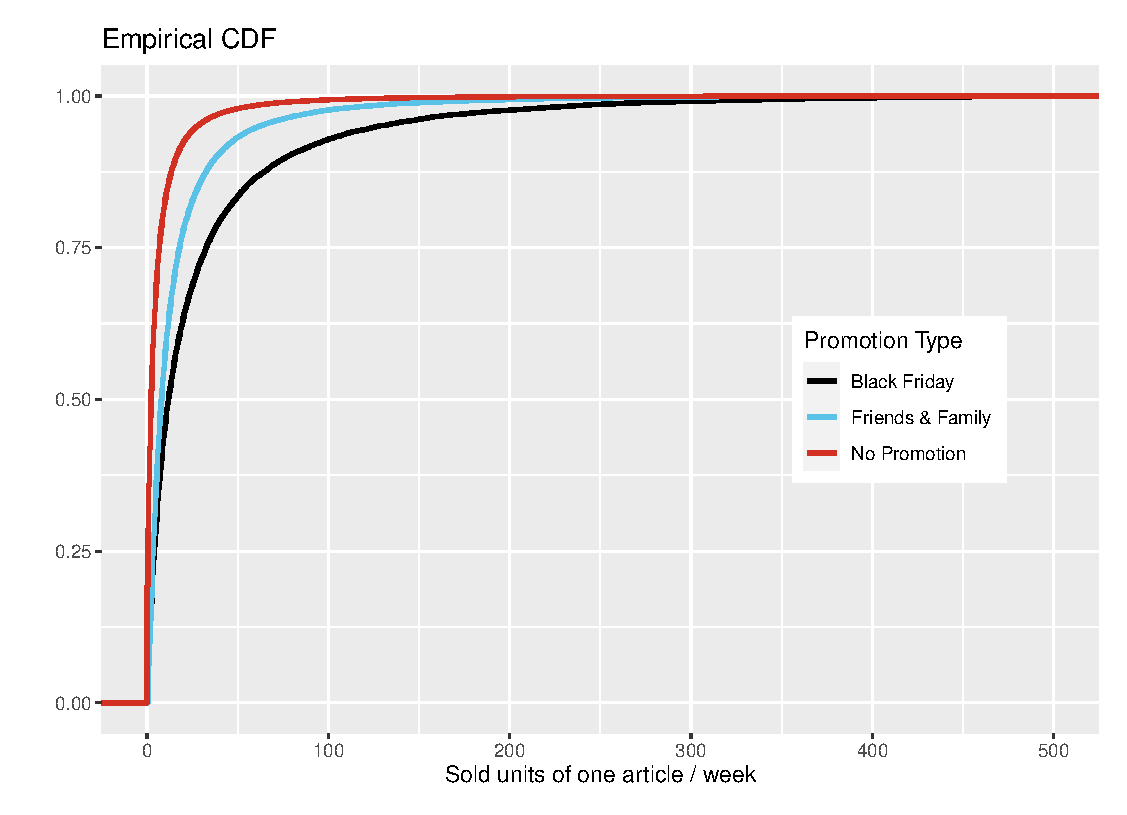
\includegraphics[width=0.65\linewidth]{figures/ecdf_all.eps}
  \caption{Empirical \ac{CDF} of all sold units per week; x-axis cut at 500}
  \label{fig:ecdf_all}
\end{figure}



Unfortunately, we cannot just remove such outliers with extreme sale numbers from the dataset, as it would produce gaps in the time series of some specific articles. Removing entire articles from the analysis is also not an option, since we would be forced to remove a lot of articles. For example, 273 articles alone would have to be removed to get rid of the highest 0.01\% of quantities (see \autoref{tab:quantiles_sold_units_week}). Besides, these extreme values might be too informative for the underlying data generating process, so we decide to keep them all.








